\documentclass[pdftex,11pt,a4paper]{article}\usepackage{graphicx, color}
%% maxwidth is the original width if it is less than linewidth
%% otherwise use linewidth (to make sure the graphics do not exceed the margin)
\makeatletter
\def\maxwidth{ %
  \ifdim\Gin@nat@width>\linewidth
    \linewidth
  \else
    \Gin@nat@width
  \fi
}
\makeatother

\IfFileExists{upquote.sty}{\usepackage{upquote}}{}
\definecolor{fgcolor}{rgb}{0.2, 0.2, 0.2}
\newcommand{\hlnumber}[1]{\textcolor[rgb]{0,0,0}{#1}}%
\newcommand{\hlfunctioncall}[1]{\textcolor[rgb]{0.501960784313725,0,0.329411764705882}{\textbf{#1}}}%
\newcommand{\hlstring}[1]{\textcolor[rgb]{0.6,0.6,1}{#1}}%
\newcommand{\hlkeyword}[1]{\textcolor[rgb]{0,0,0}{\textbf{#1}}}%
\newcommand{\hlargument}[1]{\textcolor[rgb]{0.690196078431373,0.250980392156863,0.0196078431372549}{#1}}%
\newcommand{\hlcomment}[1]{\textcolor[rgb]{0.180392156862745,0.6,0.341176470588235}{#1}}%
\newcommand{\hlroxygencomment}[1]{\textcolor[rgb]{0.43921568627451,0.47843137254902,0.701960784313725}{#1}}%
\newcommand{\hlformalargs}[1]{\textcolor[rgb]{0.690196078431373,0.250980392156863,0.0196078431372549}{#1}}%
\newcommand{\hleqformalargs}[1]{\textcolor[rgb]{0.690196078431373,0.250980392156863,0.0196078431372549}{#1}}%
\newcommand{\hlassignement}[1]{\textcolor[rgb]{0,0,0}{\textbf{#1}}}%
\newcommand{\hlpackage}[1]{\textcolor[rgb]{0.588235294117647,0.709803921568627,0.145098039215686}{#1}}%
\newcommand{\hlslot}[1]{\textit{#1}}%
\newcommand{\hlsymbol}[1]{\textcolor[rgb]{0,0,0}{#1}}%
\newcommand{\hlprompt}[1]{\textcolor[rgb]{0.2,0.2,0.2}{#1}}%

\usepackage{framed}
\makeatletter
\newenvironment{kframe}{%
 \def\at@end@of@kframe{}%
 \ifinner\ifhmode%
  \def\at@end@of@kframe{\end{minipage}}%
  \begin{minipage}{\columnwidth}%
 \fi\fi%
 \def\FrameCommand##1{\hskip\@totalleftmargin \hskip-\fboxsep
 \colorbox{shadecolor}{##1}\hskip-\fboxsep
     % There is no \\@totalrightmargin, so:
     \hskip-\linewidth \hskip-\@totalleftmargin \hskip\columnwidth}%
 \MakeFramed {\advance\hsize-\width
   \@totalleftmargin\z@ \linewidth\hsize
   \@setminipage}}%
 {\par\unskip\endMakeFramed%
 \at@end@of@kframe}
\makeatother

\definecolor{shadecolor}{rgb}{.97, .97, .97}
\definecolor{messagecolor}{rgb}{0, 0, 0}
\definecolor{warningcolor}{rgb}{1, 0, 1}
\definecolor{errorcolor}{rgb}{1, 0, 0}
\newenvironment{knitrout}{}{} % an empty environment to be redefined in TeX

\usepackage{alltt}
\usepackage{natbib}
\usepackage{wrapfig}
\usepackage[font=small,labelfont=bf]{caption}
\usepackage[none]{hyphenat}

\bibliographystyle{ecol_let}
\setlength{\parindent}{0cm}

\addtolength{\textwidth}{3cm}
\addtolength{\hoffset}{-1.5cm}

\addtolength{\textheight}{2cm}
\addtolength{\voffset}{-1cm}




\begin{document}

\title{Understanding range shift model error: The influence of generation time and rate of adaptation on species distribution model predictions.}
 \date{}
\maketitle

{\bf  Working group proposal \\}
Short title: Range shifts and rates of adaptation \\
{\it Submitted to NCEAS on August 31, 2012\\}

{\bf Principle Investigator\\}
Edmund M. Hart\\
Beaty Biodiversity Center\\
Dept. of zoology\\
University of British Columbia\\
4200-6270 University Blvd\\
Vancouver, B.C. V6T 1Z4\\
{\it ehart@zoology.ubc.ca}\\ 



{\bf Project Summary:} Species range shifts is one of the most well documented responses of species to climate change and have been modeled  using correlative niche models (species distribution models, SDMs) for more than a decade.  Because these models are based on stastical correlations between a species realized niche and abiotic variables, there is often a deviance between predictions and a species' actual distribution.  Our group will seek to understand the source of this deviance using meta-analysis.  The first goal will be to test how rates of adaptation may constrain or enhance species' ability to match climate predictions. Further exploration of patterns in model deviance can be explored once data on range predictions and extant ranges has been assembled such as model artifacts and mutualistic networks. Currently much of the data from these models is locked in the form of published figures and maps though.  Therefore a second product of our working group will be the development of a web-based data extraction tool. This will allow anyone to upload a figure and extract data from it and store that data in DataONE and other open source data sites.  This will result in a data product with a usefulness that will outlast our working group, and enable future meta-analysis.
\\
\begin{description}\itemsep1pt
\item[Start date] December 2012
\item[End date] December 2013
\item[Data release] December 2013
\item[Resubmission?] No
\end{description}

\pagebreak[4]

\section*{Problem Statement}
Species' range shifts was one of the earliest documented ecological responses to climate change \citep{Parmesan1996,Parmesan1999,Parmesan2003}.  Since the late 1990's ecologist's have been using species' distribution models (SDM's) to try and predict how those ranges will shift over the next century \citep{Davis1998,Iverson1998,Guisan2000,Peterson2001}.  These models assume that the realized niche of a species is primarily determined by climate variables \citep{Austin2002,Dormann2007}.   Ignoring physiology,  biotic interactions and rapid local adaptation has long been a source of criticisms for these models \citep{Davis1998,Pearson2003,Guisan2005,Helmuth2005}.  Aside from ignoring ecological theory \citep{Elith2009}, SDM's can show great variance in their predictive abilities \citep{Elith2006,Kearney2009,Elith2010}.  More recent SDM's have begun to incorporate mechanisms such as physiology \citep{Crozier2006,Buckley2010,Buckley2011} and  life history traits \citep{Midgley2006,Kearney2009,Poyry2009,Angert2011a} to improve fit. Including traits and physiology offers a significant improvement in model predictions \citep{Angert2011a,Buckley2011} but is nonetheless only a small percentage of unexplained variance.  Other factors may be important in explaining the error in species actual ranges and their predicted distribution. \\ 

\begin{wrapfigure}{r}{.5\textwidth}
\begin{knitrout}
\definecolor{shadecolor}{rgb}{0.969, 0.969, 0.969}\color{fgcolor}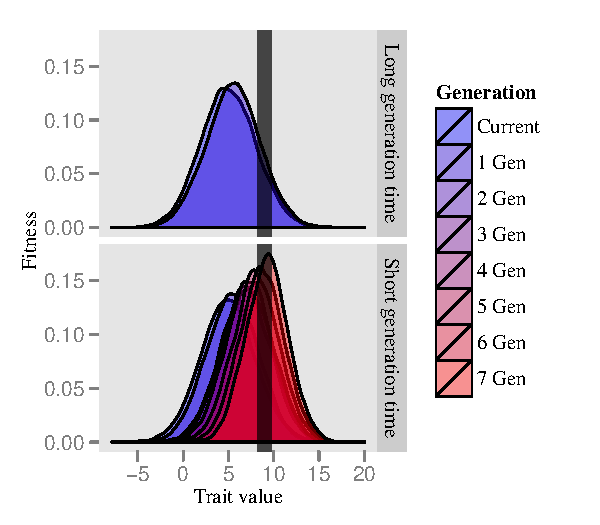
\includegraphics[width=\maxwidth]{figure/add_demo} 
\end{knitrout}

\caption{ \footnotesize{ \textit{A species with a long generation time can only complete 1 generation in a fixed time, but a short generation time can complete 7 in the same time period, rapidly advancing towards the new fitness optimum (black line)  }}\label{fig:add_demo}}
\end{wrapfigure}
Adaptation (and microevolution) to climate change is often cited as being an important facet in understanding how species will respond to climate change \citep{Visser2008,lavergne2010biodiversity,Hoffmann2011}, but it is difficult to accurately measure in the field \citep{Hansen2012}.
Despite adaptation playnig an important role in species range shifts to both current \citep{Thomas2001,Bridle2007} and historical climate change \citep{Davis2001} it is conspicuously absent from SDM's.  One way of integrating adaptation into prexisting range shift predictions is by examining the deviance between SDM predictions at the current time and the current range of species and comparing it to generation time.
Shorter generation times allow for a more rapid adaptive response to strong selective pressures \citep{Berteaux2004,Somero2010,Reed2011,Shaw2012,Walters2012}.  The first reason is that species with shorter generation times are can make use of standing additive genetic variation (Figure 1). 
For instance fur seals are predicted to be unable to adapt to rapid climate change because of long generation times, but this is not the case for other antartic species with short generation times \citep{Forcada2008}. Species with shorter generation times also have higher rates of molecular evolution due to increased mutation rates \citep{Thomas2010}.  This contributes to the amount of additive genetic variance necessary for adaptive responses to a changing environment \citep{Lande1996}.  \textbf{Our goal is to measure SDM error and investigate how rates of adaptation introduce error model prediction}\\
\\
Despite more than a decade of publications on SDM's, adaptation is still absent from most models \citep{Kearney2009}. Is there a way to analyze the vast number of existing SDM's to make inferences about the sources of error? By calculating a standard metric of error it is possible to construct models of that unexplained deviance.  The challenge is that much of the data for these models is locked in the form of published figures.  Methods already exist for data extraction such as the \textit{digitize} package \citep{Poisot2011} for R (Figure 2).  Using a combination of JavaScript and Python, we can implement a web based interface for digitization of figure data available to anyone.  

\begin{figure}[!h]
\centering
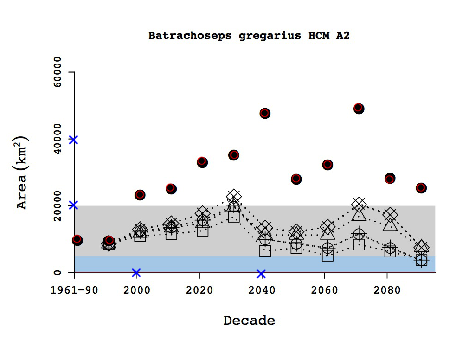
\includegraphics[height=2.2in,width=2.7in]{ExtractPlot.png}
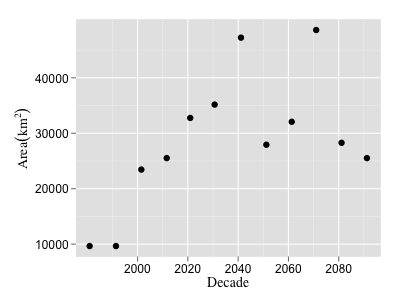
\includegraphics[height=2.2in,width=2.7in]{exportdat.png}
\caption{\textbf{Left panel: }\textit{Range shift predictions fram \citet{Early2011} of} Batrachoseps gregarius \textit{ with calibration points marked} \textbf{Right panel: } \textit{Extracted data points using the digitize package for R \citep{Poisot2011}}}

\end{figure}
 
\section*{Proposed Activities}
Our goal is to understand how rates of adaptation can cause error in SDM predictions and construct web-based tools for data collection that can be stored in open access databases for other researchers to use.  Furthermore once we collect data on error rates in SDM prediction we can test other hypotheses.

\begin{itemize}
    \item \textit{Question: Can residual error in SDM predictive models be explained by rates of adaptation?}
      \begin{itemize}
        \item Hypothesis: SDM's for species with shorter generation times should have greater error rates because they can rapidly adapt to new invaders and novel climate scenarios at the trailing edge of their distribution.  Therefore they are less likely to track their current shifting climate
        \end{itemize}
    \item \textit{Software product: A web-based interface for data extraction of digitized figures.}
      \begin{itemize}
        \item An open source tool that will allow anyone to extract data from digital figures including: scatter plots, bar charts and georeferencable maps.  The interface will store the data at DataONE which can then be used for any future meta-analysis.
        \end{itemize} 
\end{itemize}

\textit{Error analysis} \\
Error can be calculated in three ways: difference in area of occupancy, difference in expanding front, and difference in trailing edge.  The first two are the most common and we will have the largest sample from these.  All these can be theoretically be compared by converting them to Z-scores and calculating a standard error statistic such as root-mean squared error.  Once we have quantified error, we can construct mixed effects models with error as the response variable.  The predictor of interest will be generation time.  Other variables will also be included, for instance it's known that different SDM contstruction methods have differences in performance \citep{Elith2006, Elith2010}.  Using this framework we can add other covariates into our models to control for modeling artifacts. 





\bibliography{NCEASbib}
\end{document}


